\documentclass[12pt]{report}
\usepackage[utf8]{inputenc}
\usepackage{graphicx}
\usepackage{float}
\usepackage{pgfgantt}
\usepackage{hyperref}
\usepackage{algorithm2e}
\usepackage[left=2cm,right=2cm,top=2cm,bottom=2cm]{geometry}

\usepackage[toc]{glossaries}
\usepackage{appendix}

\usepackage{mathptmx}
\makeglossaries


% Comments
\usepackage{color}
\usepackage[normalem]{ulem} %pour le format barré
\newcommand{\hcp}[1]{\textcolor{blue}{[#1]}}
\newcommand{\hcr}[2]{\textcolor{red}{\sout{[#1]} - \textcolor{blue}{ [#2]}}}
\newcommand{\hc}[1]{\textcolor{red}{[#1]}}
\newcommand{\hcc}[1]{\textcolor{green}{Pour info - [#1]}}
\usepackage{biblatex}
\addbibresource{references.bib}

\begin{document}
	\begin{titlepage}
		
		\newcommand{\HRule}{\rule{\linewidth}{0.5mm}} % Defines a new command for the horizontal lines, change thickness here
		
		\center 
		\HRule \\[0.4cm]
		{ \huge \bfseries Report \\Representation and relative positioning from visual information}\\[0.4cm]
		\HRule \\[1.5cm]
		
		\begin{minipage}{0.4\textwidth}
			\begin{flushleft} \large
				\emph{Submitted by:}\\
				\textsc{Asma BRAZI}
			\end{flushleft}
		\end{minipage}
		~
		\begin{minipage}{0.4\textwidth}
			\begin{flushright} \large
				\emph{Supervised by:} \\
				\textsc{Cédric HERPSON}\\
			\end{flushright}
		\end{minipage}\\[4cm]
		
		
		{\large Laboratory of Computer Sciences, Paris 6 \\ Sorbonne University - Faculty of Sciences and Engineering}\\[3cm] 
		{\large June - July 2019 }\\[3cm] 
		
\includegraphics[width=0.6\textwidth]{res/logo.png}\\[1cm] 
		\vfill % Fill the rest of the page with whitespace
		
	\end{titlepage}
	

	\chapter{Abstract}
	
	\paragraph{}
	We carried out our internship at the Laboratory of Computer Sciences, Paris 6 (LIP6) under the supervision of M. Cédric Herpson, from June 3rd, 2019 until July 26th, 2019. The internship was mainly considered as a continuation of works that we carried out during a university project (PANDROIDE) in our first Master's degree. 
	
	\paragraph{}
	Our previous works presented a naive approach of object recognition and exploration strategy that allowed an autonomous robot with a camera to roughly build its environment. The environment is closed and composed of walls where the robot was able to locate itself. In addition, we could ask the robot to search for a specific object, and the robot was able to accomplish that task. Nevertheless, the conducted works assumed some hypotheses which did not make the exploration strategy generic.
		
	\paragraph{}
	During this internship, we focused the most on improving the exploration strategy, to no longer depend on certain hypotheses. For example, in our previous works, we had some specific objects placed on corners to indicate to the robot that there were a corner at this spot. This hypothesis allowed the robot not to perform image processing to detect corners. 
	
	\paragraph{}
	Our new strategy does not depend anymore of these objects. But, it exploits some visual information as contours. Also, the information provided by the robot's sensors is taken into account. We developed so a strategy where no knowledge of the environment is necessary, and no hypothesis helping the robot building its environment are considered.
	
	\chapter{Acknowledgments}

	\begin{center}
		
	
	I would like to deeply thank my supervisor, M. Cédric Herpson, for his guidance and help, his presence and his trust in me to lead the initiative in my work. 
	
	I can say that I have been truly lucky to have M. Cédric Herpson as a supervisor who cared so much about my work, although he had a lot of work ahead of him. 
	\end{center}
	
	\tableofcontents
	\chapter{Introduction}
	\paragraph{}
	When an autonomous robot navigates in a structured or unstructured environment, it should be able to build a map representing this environment, to localize itself in it, and to define a safe path to move from a place to another one.
	
	\paragraph{}
	There are a varied applications of the robot navigation. Such as surveillance, cleaning, transportation tasks...etc. As a result, the number of contributions of researchers in this field keeps going up \cite{bonin-font_visual_2008}.
	
	\paragraph{}
	Our project aims to enable the Thymio robot\footnote{An educational programmable robot} with a camera to build roughly  its environment. The environment is closed and it is composed of walls where the autonomous robot is able to locate itself. 
	
	\paragraph{}
	Unlike our previous work where we had some landmarks helping the autonomous robot in the detection of corners, we develop throughout the internship a more generic strategy. The autonomous robot is based only on its sensors and camera to build the environment.
	
	So with this strategy, the robot can manage to build its entire environment autonomously.
	
	
	\section{Outline of this report}
	\paragraph{}
	The remaining chapters are organized as follows:
	\begin{itemize}
		\item Chapter 4: Summarize of the state of art.
		\item Chapter 5: Explanation of the solution.
		\item Chapter 6: Discussion and test of the solution.
		\item Chapter 7: Conclusion and suggestion of future works.
	\end{itemize}: 
	
	
    \chapter{Reviews of Existing Work}
	
	\paragraph{}
	The main purpose of our works is to improve the functionalities developed previously. These functionalities allowed the autonomous robot to move in its environment (A rectangular room) and to explore it. 
	
	\paragraph{}
	The visual information brought by the exploration is used to build a virtual 3D representation of this environment, and to recognize a target object. The target object is an object from the knowledge database. It is specified by the user, at the launching of the application.
	
	\paragraph{}
	In short, our previous strategy can be summarized as follows:
	\begin{itemize}
		\item At each move, the autonomous robot took a picture and analyzed it.
		\item The analysis of the picture brought a new knowledge to the autonomous robot.
		\item With this new knowledge, The autonomous robot was in one of these situations:
		\begin{itemize}
			\item The target was detected and the exploration ended.
			\item The four walls was explored and the target was not detected. So, the exploration ended.
			\item A corner was detected. As a result, the autonomous robot went on the next wall.
			\item Anything was detected, the autonomous moved to the next part of the same wall.
		\end{itemize}
		\item Repeat until the exploration ended.
	\end{itemize}

	\paragraph{}
	However, we assumed some hypotheses which facilitated the exploration process. For example, we placed some objects (landmarks) in each corner of the environment and every time the autonomous robot met these objects, it concluded that this was a wall end. So the autonomous robot relied on these objects to decide whether or not it finished exploring the current wall.
	
	Otherwise seen, as long as the autonomous robot did not meet a landmark, then it continued moving forward assuming it is the same wall.
	
	\paragraph{}
	Also, another hypothesis is when the autonomous robot did not detect anything, and it assumed that it was the continuation of the current wall. Such a hypothesis may be hard to omit if we want to adjust the strategy to be usable in a more complex environment. A complex environment may be a room with corridors. In that case, a corridor may be ignored, because the autonomous robot only took into account the presence of objects for the decision and not the structure of the environment.
	
	\paragraph{}
	To no longer depend on these hypotheses, our works present another manner to build the environment. Firstly, we do not assume anymore having a rectangular room as environment, but we build a strategy which may work independently of the environment structure. 
	\paragraph{}
	Than, the autonomous robot does not suppose the presence of a wall by detecting one of its corners. Instead, it extracts the contours of the environment with whom the autonomous robot decides if it is in front of a close/far wall, if there is a wall behind them...etc.
	
	By this way, the autonomous robot gathers the analysis's results to estimate the dimensions of the walls.
	
    \chapter{Realization}
    \paragraph{}
    We suppose that the autonomous robot is situated in a closed environment, and it has been informed about the target object to search. 
	\section{Exploration strategy}
	 \subsection{Image processing}
	 \paragraph{}
	 The first task of the autonomous robot is to represent roughly the environment, using visual information. For walls detection, we distinguish three types of segments on the picture taken by the autonomous robot:
	 \begin{itemize}
	 	\item Vertical segment which makes almost 90 degrees with the X-axis.
	 	\item Horizontal segment which makes almost 0 degree with the  X-axis.
	 	\item Diagonal segment which makes an acute angle with the X-axis.
	 \end{itemize} 
	 
	 
	 \paragraph{}
	 In the sections to come, we present the different strategies we have developed and the one we have particularly kept.
	 
	 \subsubsection{Corners-based detection}
	 \paragraph{}
	 We have begun with a strategy based on corners detection. Where we kept the same exploration strategy as in our previous works. But, we replaced only the part of corners detection. So instead of detecting a specific objects substituting the corners, we tried two methods. We developed an approach based on \textit{segments intersection} and we used a preset method from OpenCV for \textit{corners detection}. These two methods were used under a certain constraints, to decide whether it is a corner or not.
	 \paragraph{}
	 Defining these constraints is not that easy. For example, it is getting arduous if we have a textured floor or walls. So the method considers all the intersection points situated on the walls and on the floor as corners. 
	
	 Also, if the floor and the walls have almost the same color, the segment separating the wall from the floor may not be detected.
	 
	 As a result, these methods detect a lot of features which are not all correct corners.
	 
	 \paragraph{}
	 On the other hand, if we assume that corners are situated in most cases on the bottom of the image, this assumption becomes incorrect if the autonomous robot is so far from the corner. In this case, the corner is situated on the top of the image. The figure below demonstrates that:
	 	\begin{figure}[H]
	 	\begin{center}
	 		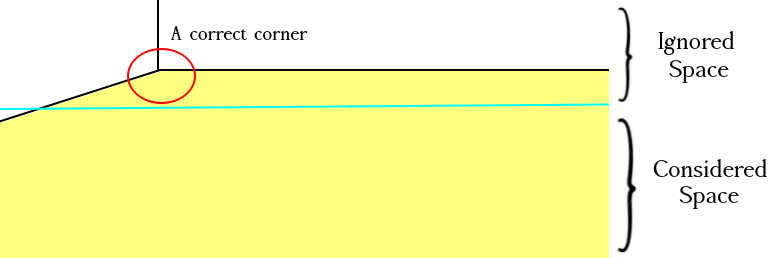
\includegraphics[scale=0.6]{res/start1_c1.png}
	 		\caption{An ignored corner because of the corners placement constraint}
	 	\end{center}
	 \end{figure}
	 \paragraph{}
	 As a result, this corner will be ignored as it is not situated on the bottom of the image.
	 
	 \paragraph{}
	 These particular pictures taken by the autonomous robot make the strategy not really captivating, because it is sensitive to the autonomous robot's position.
	 
	 \subsubsection{Non corners-based detection}
	 \paragraph{}
	 After encountering some difficulties to detect the right corners, we decided to ditch this strategy because it was impractical. 
	 
	 \paragraph{}
	 The next idea is to consider the segments on the 3 axis X,Y and Z. The vertical (resp. horizontal) segments are used to estimate the walls height (resp. width). However the diagonal segments indicate that there is a depth. Knowing that a certain depth exists on the image, guarantees to the autonomous robot that there is still space between them and the wall in front. So, it can always move forward.
	  
	  \paragraph{}
	  We have used the \textit{Line Segment Detector} algorithm (LSD) to detect straight contours on the image \cite{grompone_von_gioi_lsd:_2012}. At each pixel of the image, LSD estimates the angle of the gradient. After that, the pixels sharing nearly the same angle of gradient are merged into regions. The connected regions are called \textit{line support regions}. Then, the algorithm keeps some of these \textit{line support regions} to be a \textit{line segment}.
	  
	  \paragraph{}
	  The picture below shows an image on which the LSD was applied and as a result, the \textit{line support regions} that were detected.
	  	\begin{figure}[H]
	  	\begin{center}
	  		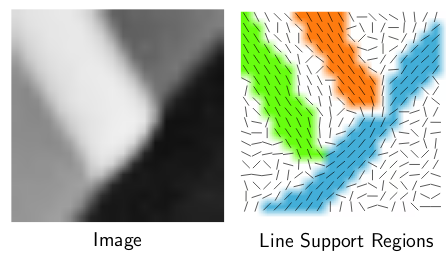
\includegraphics[scale=0.6]{res/lsr.png}
	  		\caption{Line Support Regions. Adapted from "Rafael Grompone von Gioi, Jérémie Jakubowicz, Jean-Michel Morel, and Gregory Randall, LSD: a Line Segment Detector, Image Processing On Line, 2 (2012)" }
	  	\end{center}
	  \end{figure}
  \paragraph{}
  So, on each picture taken by the autonomous robot, we apply LSD to obtain segments. After that, the segments are classified into groups: the verticals, the horizontals and the diagonals, up to a certain tolerance $\epsilon$. Each group of segments is used for a certain purpose for the navigation. Then, in each group, we merge the closet segments up to a certain tolerance $\lambda$, in order to get a longer segments, and we keep only the longest one from each group at the end. 
  
\paragraph{}
The horizontal segments which are situated on the top of the image are ignored. We assume that theses segments represent a ceiling. We do not risk anything by ignoring theses segments because, even if the segments represent a frontier between the floor and far wall. We built a strategy where the autonomous robot does not build a wall unless it is close to it.
    \subsection{3D map building}
    
    \paragraph{}
    We remind that our goal is to build a rough 3D representation of the environment and look for the target object. We represent the environment by defining the walls composing it. The detection of walls is based on LSD's segments.
    
    \paragraph{}
    Depending on the autonomous robot's position, the picture obtained may be in one of the general cases showed in the picture below. 
    
    
    	\begin{figure}[H]
    	\begin{center}
    		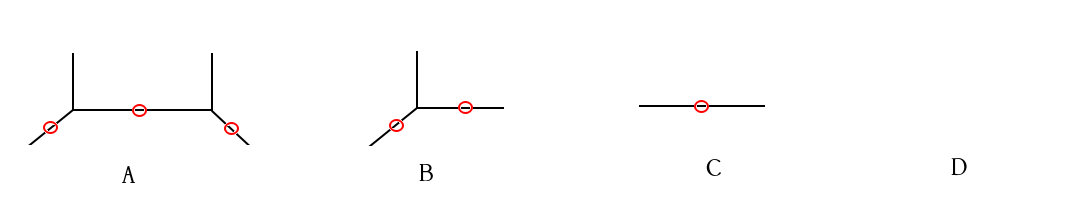
\includegraphics[scale=0.65]{res/cases_seg.png}
    		\caption{Walls detection depending on the robot's position}
    	\end{center}
    \end{figure}
 \paragraph{}
 The useful information that we can retrieve from each case is as follows:
 \begin{itemize}
 	\item Case A: 3 types of segments are detected, an horizontal one and 2 diagonals on 2 opposing walls.
 	\item Case B and C: 2 types of segments (horizontal and diagonal) sharing an endpoint are detected.
 	\item Case D: An horizontal segment is detected.
 	\item Case E: Any segment is detected.
 	
 \end{itemize}
 \paragraph{}
 We mention that the vertical segments are used only to set the height of walls, they are not used in the exploration strategy because the autonomous robot is moving only along the X and Z axis.
 \subsection{Navigation}
     \paragraph{}
 Navigation is the determination of an adequate and secure path for the autonomous robot, to move from a starting spot to a target one \cite{bonin-font_visual_2008}.
 \paragraph{}
 On the basis of visual information, the autonomous robot is able to define its next decision. The decision may be to:
 \begin{itemize}
 	\item Stop if the target has been found or if the robot has explored the entire environment, without spotting the target.
 	\item Avoid obstacles.
 	\item Move back, move forward and rotate to continue exploring.
 \end{itemize}

\subsubsection{Obstacle avoidance}
\paragraph{}
In our previous work, when the autonomous robot decided to move forward, it did not check progressively while moving whether there is an obstacle or not. But, it verified if there is an obstacle when it stopped moving. The drawback of such a decision is that the autonomous robot was not able to distinguish between its last position at the end of the movement and its position at the first moment when it met the obstacle. As a result, the autonomous robot thought that it traveled the entire distance.

\paragraph{}
In our new strategy, the autonomous robot stops as soon as it detects an obstacle. Its sensors may detect the presence of an obstacle at almost 10 centimeters. When the autonomous robot stops, the real distance traveled is returned. If there were no obstacles, the distance would be entirely traveled.
\subsubsection{Strategy}
\paragraph{}
As there are a lot of cases of movements according to the visual information, we try to summarize these cases using an activity diagram shown in the figure below. In this diagram, the green boxes represent a physical movement done by the autonomous robot, and the blue cases represent treatments. 

\paragraph{}
We assume that the user has already mentioned the name of the object to find, and that the robot is situated in a close environment.

If we start with the initial point of the diagram, we can see that the autonomous robot begins by taking a picture and analyzes it. After that, it extracts the visual information from the picture taken and sends them to the computer, where the orders of movements are given. 

From the collected information, if the target has been found, the autonomous robot stops. Otherwise, If there are any segments detected, each of these segments is represented by a wall and added to the 3D map.
\paragraph{}
At the end of the treatment, a movement is ordered to the autonomous robot (rotate, move back...etc). Then, it regains from the beginning until it stops.
\newpage
	\begin{figure}[H]
	\begin{center}
		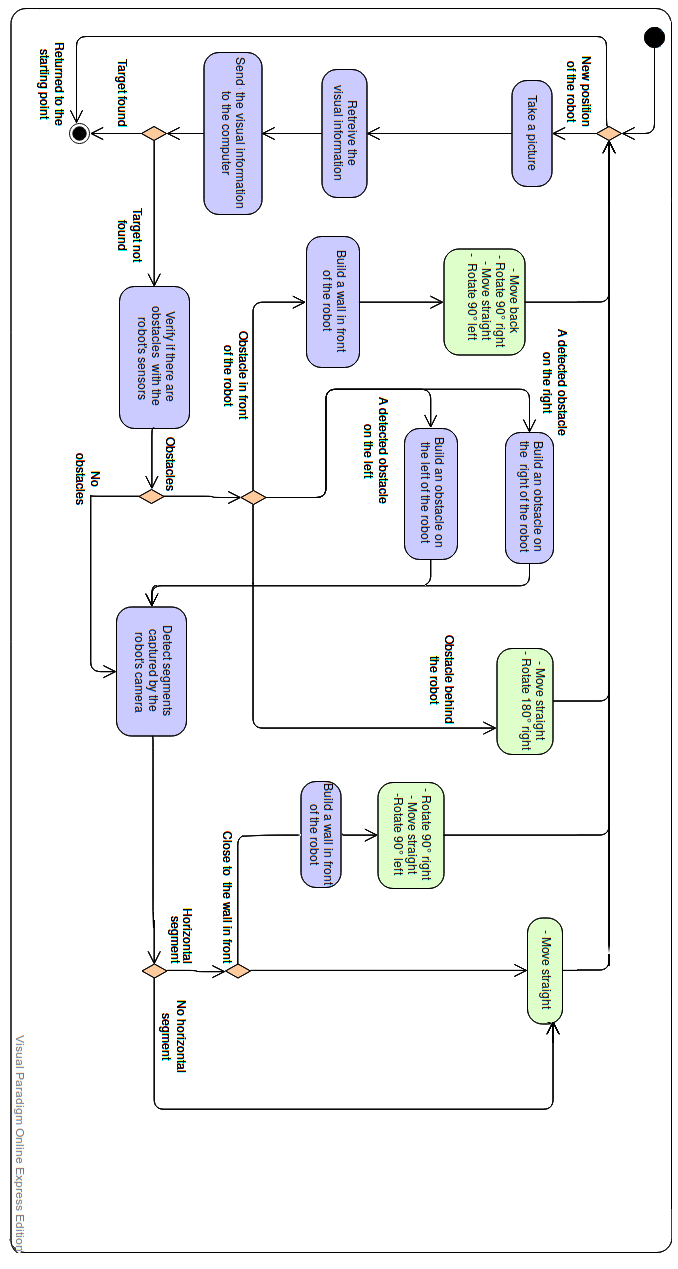
\includegraphics[scale=0.55]{res/order_processing.png}
		\caption{Activity diagram of the exploration strategy}
	\end{center}
\end{figure}
\newpage
	

	\chapter{Testing}
	\paragraph{}
	\section{Environment plan}
	We chose an environment which contained corridors, obstacles, textured walls, different level of light and different types of door. Such an environment is interesting to reveal the robustness of the strategy.
		
	\paragraph{}
	When launching the application, the target object is filled in. Then, the autonomous robot is going to build progressively its environment while searching the target object. The picture below represents the environment plan.
	\begin{figure}[H]
		\begin{center}
			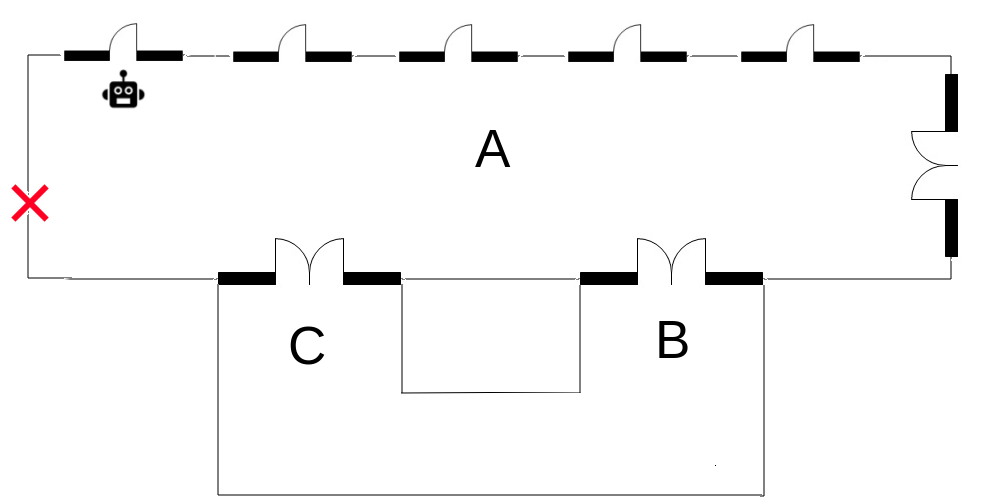
\includegraphics[scale=0.55]{res/plan.png}
			\caption{Plan of the environment}
		\end{center}
	\end{figure}
	\paragraph{}
	We can see that the plan is composed of a principal corridor (A) with 5 simple doors and 3 double-doors. There are two double-doors in front of the simple ones which lead to 2 other corridors (B and C). Than, the autonomous robot is represented by a robot symbol and it is in front of a door in the principal corridor. The autonomous robot will try to find the target object which is represented by a red cross.

	\section{Image processing}
	\paragraph{}
	In this section, we present the environment structure detection in different spots. We precise that the vertical segments are green, the horizontal ones are red and the diagonal ones are blue.
		\begin{figure}[H]
		\begin{center}
			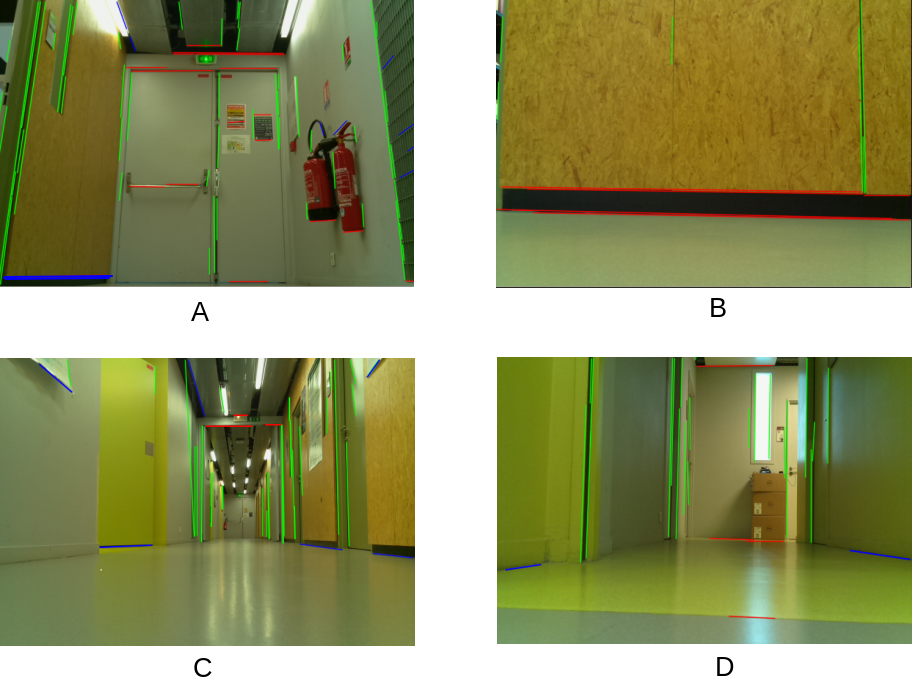
\includegraphics[scale=0.70]{res/img_proc.png}
			\caption{Segments detection testing}
		\end{center}
	\end{figure}
	\paragraph{}
	The segments shown in the figure above are not all considered. For example for those which are on the top of the image (On the ceiling) are ignored by the algorithm later. Also, we remind that we keep only the longest segment from each category (Horizontal, vertical and diagonal).
	\paragraph{}
	The weak point of this algorithm is when the floor and the wall have almost the same color, we can see that in the figure C. However the algorithm encounters any difficulties while detecting segments on the brown wall. But, it fails at the detection of the frontier between the gray wall and the floor.
	
	\paragraph{}
	Another weak point may be noticed is when there is not enough lights in the room, as in the figure D. The wall on the left is nearly dark. Moreover both  the wall and the floor are gray.
	
	\paragraph{}
	Beyond these weak points, the algorithm is able to extract the most important contours from the image, which remains sufficient for the decision. 
	\section{3D map building}
	\paragraph{}
	The picture below represents a 3D map representation of the environment at the end of the exploration. We precise that the environment has been built at a scale of 1/100 centimeters, hence the eventual impression that the walls are very offbeat.
	\paragraph{}
	At the beginning and as shown on the plan, the autonomous robot is in front of the first simple-door from the left. As mentioned in the strategy that the autonomous robot goes always right while exploring the wall, the autonomous robot explores almost all the environment before finding the target object.
	\begin{figure}[H]
		\begin{center}
			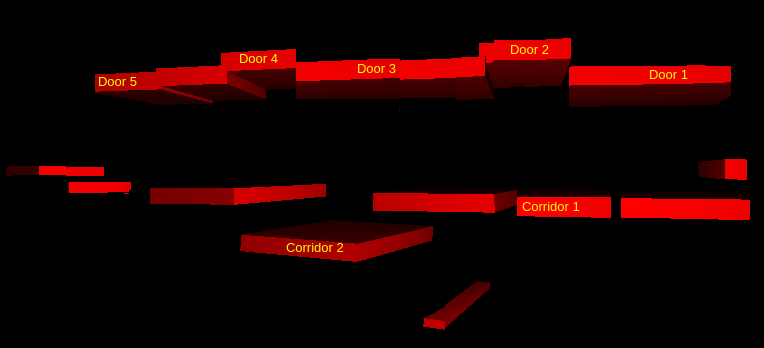
\includegraphics[scale=0.90]{res/3D_recons.png}
			\caption{3D map building of the environment}
		\end{center}
	\end{figure}
	
	\paragraph{}
	Now, we detail the 3D representation and we explain some details about it:
	\begin{figure}[H]
		\begin{center}
			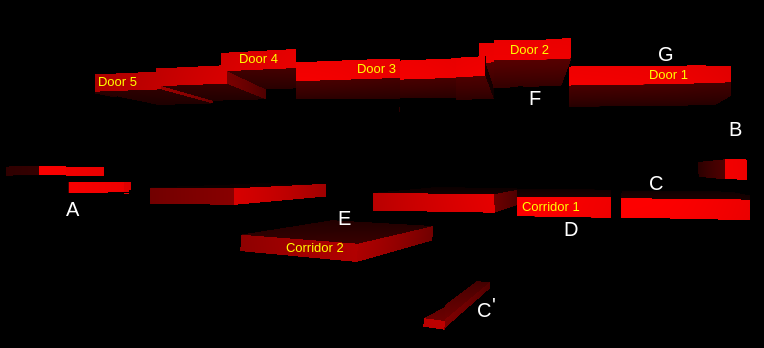
\includegraphics[scale=0.90]{res/3D_recons_det.png}
			\caption{Discussion of the environment representation}
		\end{center}
	\end{figure}
	\begin{itemize}
		\item Case A: The autonomous robot is close to the opposite wall and it travels a short distance to explore a new part of the same wall. So, the recovery phenomenon can take place because a part of the wall explored at the first spot remains in the field of view of the autonomous robot at the second spot. As a result, we get two bunk walls.
		\item Case B: There is a gap between the double-door and the floor. As a result, the segment separating the wall and the double-door may sometimes not be detected. According to the strategy, the autonomous robot moves forward and meets an obstacle (The double-door). Consequently, it draws a wall with a small width and continue exploring the rest of the environment. The picture below shows that specific case.

			\begin{figure}[H]
			\begin{center}
				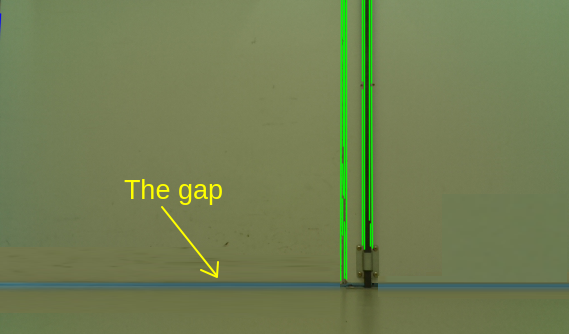
\includegraphics[scale=0.50]{res/no_segment.png}
				\caption{The grap between the double-door and the floor case}
			\end{center}
			\end{figure}
		We do not consider the vertical segment (In green)  and conclude that it is a wall, because the height does not guarantee the presence of a close wall. It may represent the height of an entire wall which is very far from the autonomous robot.
		
		
		\item Case C: At that spot, there is a big ventilation grid (fig. below). The autonomous robot detects one of the horizontal segment of the ventilation and considers it as a width of the wall in front. Unfortunately, the ventilation grid is lifted off the ground. Thus, The autonomous robot concludes that it's a border between the ground and a wall away from them, and places a far wall at C'.
	\begin{figure}[H]
	\begin{center}
		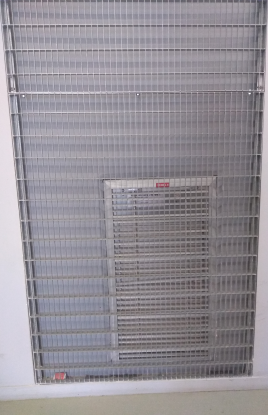
\includegraphics[scale=0.60]{res/grid_vent.png}
		\caption{Ventilation grid obstacle}
	\end{center}
\end{figure}
	
		\item Case D: We turn off the lights of the corridor 1 to see how the autonomous robot behaves. Naturally, the corridor is dark on the picture at this spot. As a result, any segment of the corridor 1 is detected. But, the autonomous robot is located in the principal corridor where the lights is on, and the floor of the principal corridor and the corridor 1 had different colors. Consequently, The limit between the two floors is detected as an horizontal segment and the autonomous robot believes that it is a wall.
		\begin{figure}[H]
			\begin{center}
				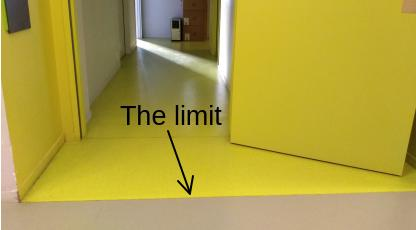
\includegraphics[scale=0.80]{res/limit_cor.jpg}
				\caption{Two floors with different colors case}
			\end{center}
		\end{figure}
	\item Case E: We keep the lights on in the corridor 2. We notice that the far wall of the corridor 2 is detected. Normally, the autonomous robot should move forward, because it detects too the diagonal segments which guarantee the presence of a depth. Nevertheless, we have omitted from our strategy the consideration of diagonals in decision. Because, a shadow was detected once as a diagonal in a case where there were any depth, ans this misleads the autonomous robot.
	
	\item Cases F and G: Bearing in mind the margin of error in rotation and movement, the closed doors 2 and 4 are detected properly. However the doors 1, 4 and 5 may be missed and considered as a walls.
	\end{itemize}

	\paragraph{}
	After testing the strategy in a complex environment contrary to a simple rectangular room, we can judge that the strategy remains more generic and does not depend anymore of the environment structure, a markers objects substituting corners...etc. Also, we arrived at a precision at a scale of 1/100 centimeters, and the same exploration strategy run at a scale of centimeters would have a smoother representation.


	\chapter{Conclusion, Limitation and Future work}
	\paragraph{}
	During our internship, we focused the most on how to make the exploration strategy more generic. We can be somewhat satisfied with the work that has been done so far, comparing to our previous works and with respect to the internship's duration.

	\paragraph{}
	Nevertheless, we suggest some ideas of how our works can be improved:
	\begin{itemize}
		\item Multi-agent exploration: Instead of exploring the environment with only one autonomous robot, we can imagine having a group of autonomous robots doing so. In this case, the communication between the robots is to develop.
		\item 3D object recognition: The current database contains only a 2D models. Works could be done in that field to manipulate a 3D models instead of 2D ones. This facilitates the recognition of the object at any views. Because now, the autonomous robot should be in front of the object to be able to recognize it.
		\item 2D/3D object detection with Deep Learning: If the database becomes large, the current object recognition may take a long time to analyze the picture. Because it tries to match the picture with each element of the database.
		\item Smooth environment representation: In our exploration strategy, a huge wall may be explored progressively. As a result, a parts of that wall are built side by side instead of building that wall as one piece. An improvement would be to merge that blocks of walls into one wall.
		
	\end{itemize}
\paragraph{}
To conclude, having an internship at LIP6 and being guided by an amazing supervisor provide us with unique opportunities for personal growth. I did not expect at my first day that I will learn as much knowledge at the end. Well, we come out of our internship further strengthened. 
	\chapter{References}
	\nocite{*}
    \printbibliography
\end{document}